\subsection{实验目的}
设计和使用低通滤波器,滤除分布在图像中的高斯白噪声。
\subsection{实验原理}
\subsubsection{高斯白噪声}
高斯白噪声是一种理想的噪声模型。高斯白噪声中,噪声振幅值是服从正态分布的。
\[ f(x)=\frac{1}{\sqrt{2\pi}\sigma}\mathrm{e}^{-\frac{(x-\mu)^2}{2\sigma^2}} \]
它的振幅分布直方图如下图\ref{fig:gwnhistogram}所示。
\begin{figure}[H]
	\centering
	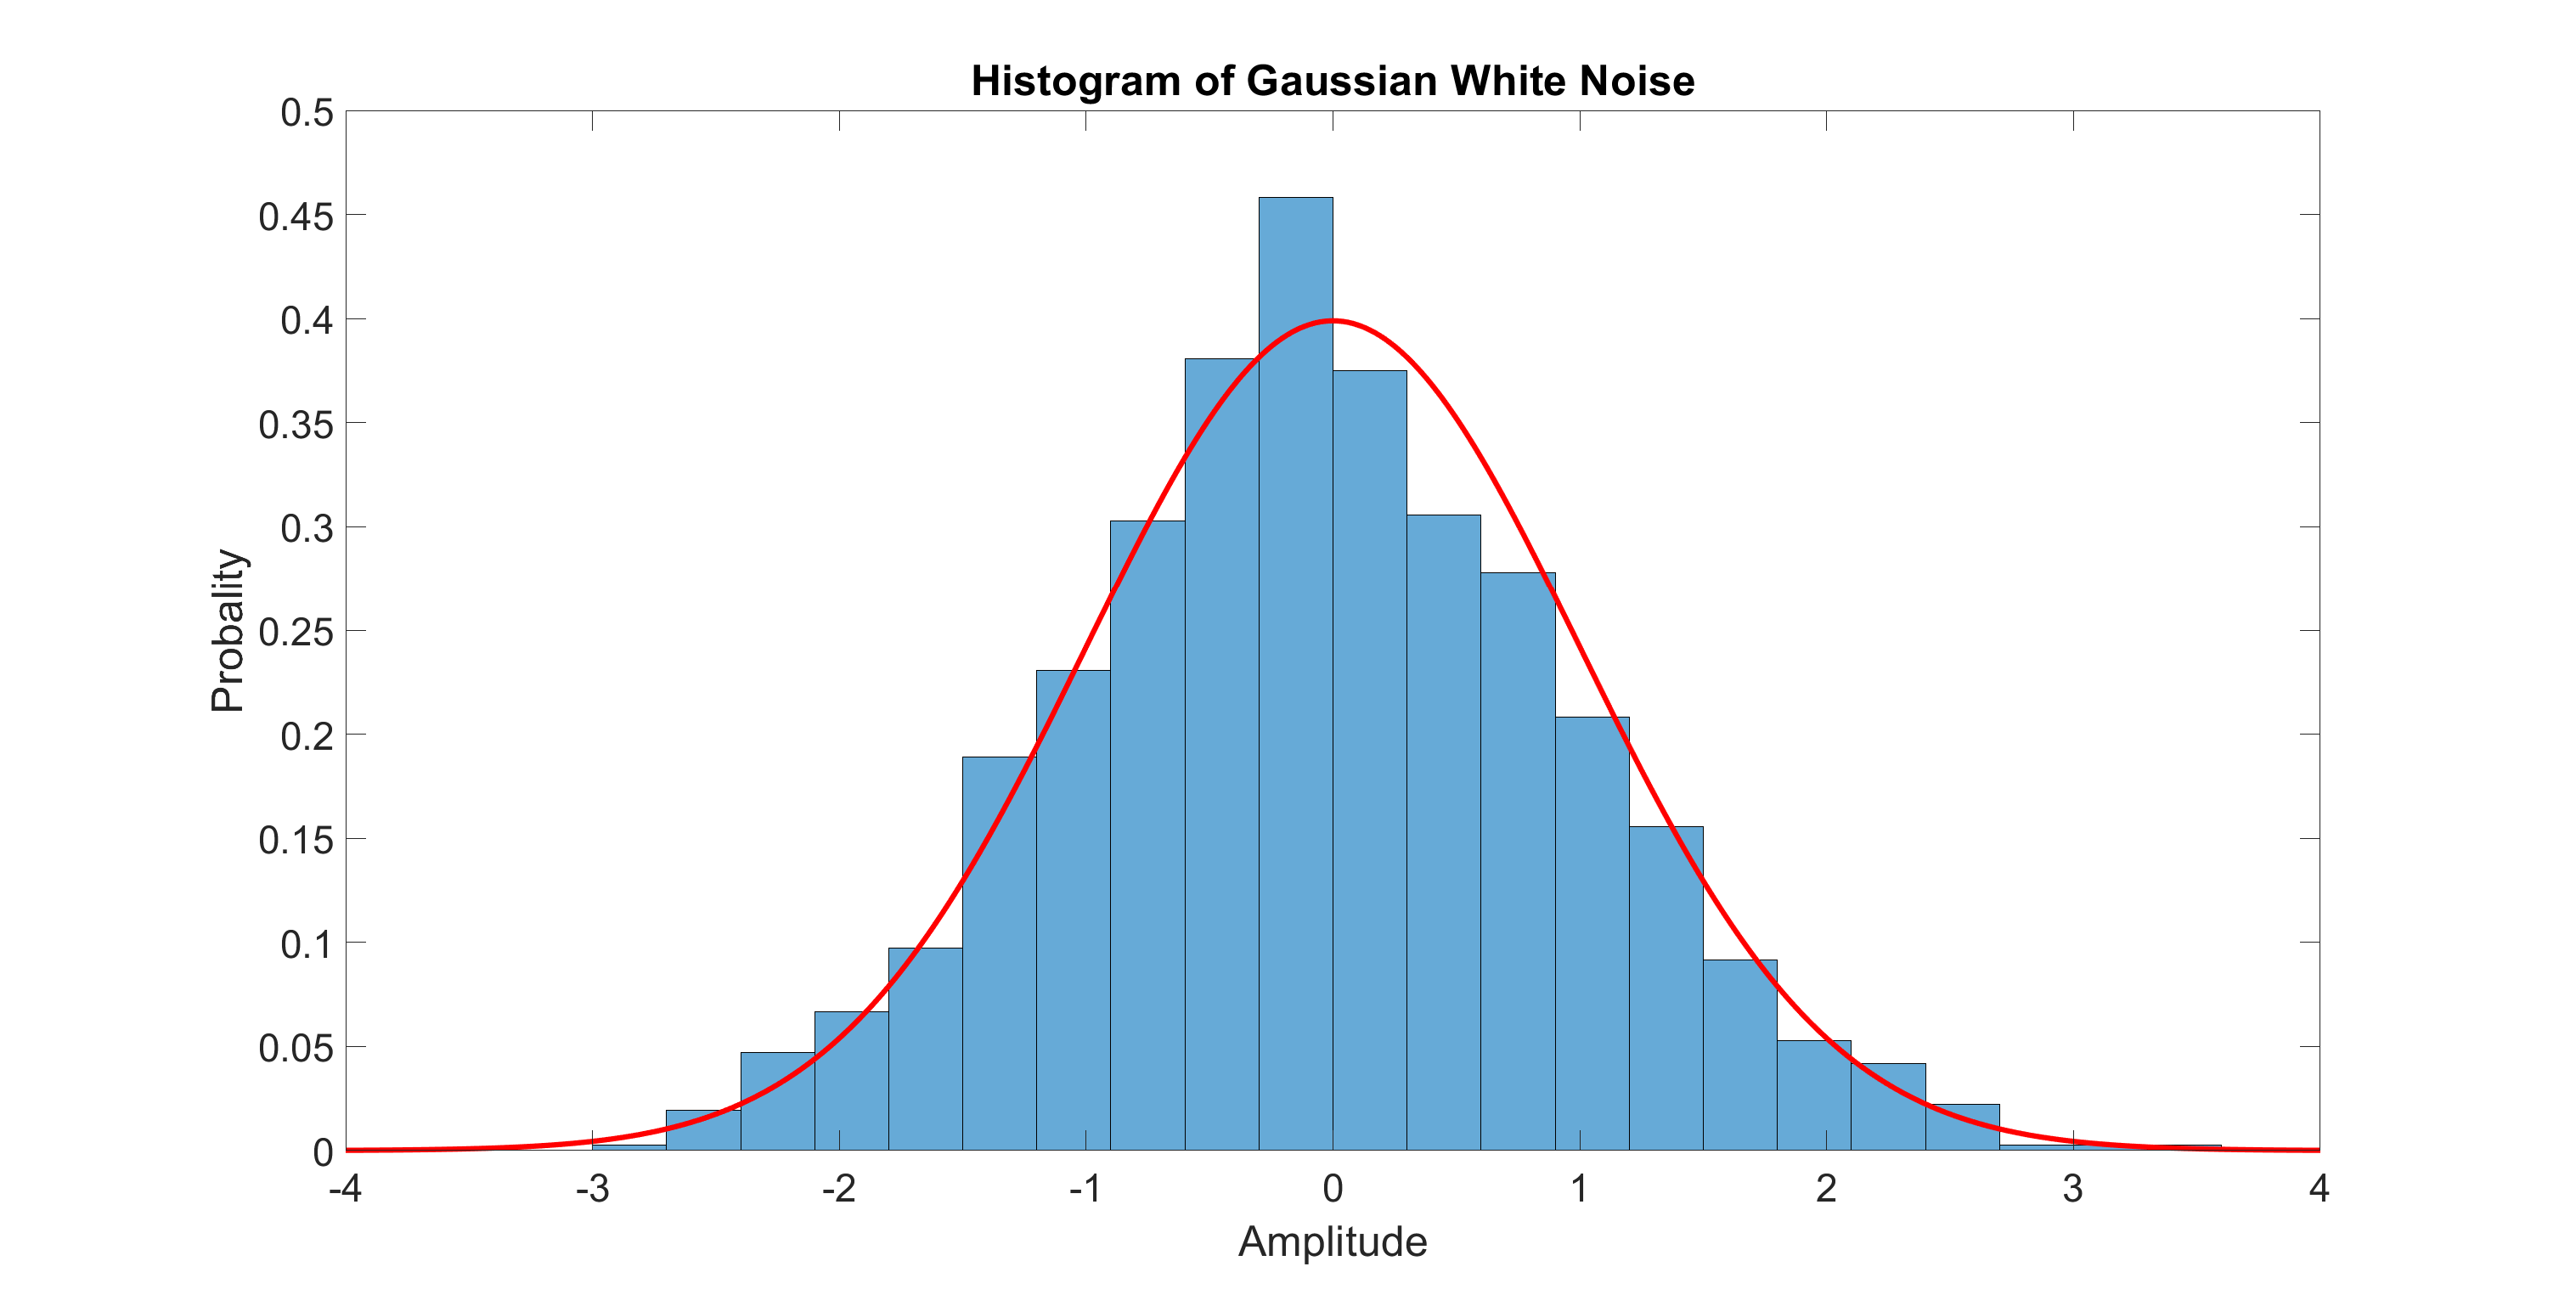
\includegraphics[width=0.7\linewidth]{figure/gwn_histogram}
	\caption{高斯白噪声幅度概率分布}
	\label{fig:gwnhistogram}
\end{figure}

它的功率谱是在频域内均匀分布的。
\subsubsection{傅里叶变换}
\subsubsection{低通滤波器}
\subsection{实验流程}
\subsection{实验程序}
\subsection{实验结果和分析}